\chapter{Wstęp}

\section{Opis procesu}

\paragraph{}
Proces badany w pracy to linia montująca płyty drukowane do finalnych produktów. Sam proces składa się z kilku etapów:
\begin{enumerate}
	\item Pobranie potrzebnych elementów elektronicznych z magazynu.
	\item Uzbrojenie pick\&place w wymagane elementy.
	\item Pobranie gotowych płyt PCB (ang. Printed Circuit Board).
	\item Ręczne nałożenie pasty lutowniczej za pomocą sitodruku
	\item Uruchomienie procesu montażu elementów na maszynie pick\&place
	\item (Opcjonalnie) Umieszczenie ręczne elementów
	\item Przeprowadzenie procesu lutowania w piecu.
	\item (Opcjonalnie) Lutowanie ręczne
	\item (Opcjonalnie) Kontrola gotowej płyty PCB
\end{enumerate}

\paragraph{}
Ograniczenia procesu:
\begin{itemize}
	\item Wszystkie procedury muszą być wykonane w ustalonej kolejności
	\item Dla płyt dwustronnych należy powtórzyć sekwencję od punktu 4 do punktu 7
	\item Pick\&place może obsługiwać tylko jedną płytę PCB
	\item Piec lutowniczy może lutować kilka płyt drukowanych (ilość jest zależna od rozmiaru płyt)
\end{itemize}

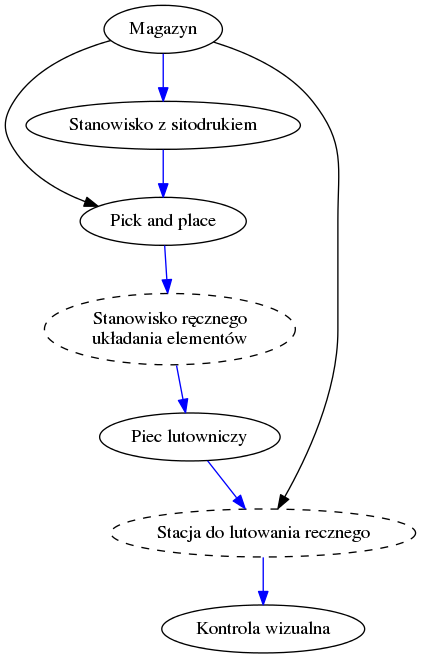
\includegraphics{chapters/graph.png}